\documentclass[a4paper,oneside]{Tptesi2}

% --- IMPOSTAZIONI LINGUA E TESTO ---

\usepackage[utf8]{inputenc}
\usepackage{csquotes}         % Utile per la corretta gestione delle virgolette in inglese

% --- PACCHETTI STANDARD ---
\usepackage{listings}
\usepackage{amsmath,amssymb}
\usepackage{verbatim}
\usepackage{indentfirst}
\usepackage{subfigure}
\usepackage{algorithmic}
\usepackage{framed}
\usepackage{rotating}
\usepackage{cite}
\usepackage{tikz}
\usepackage{textcomp}

% Use a small font for the verbatim environment
\makeatletter  % makes '@' an ordinary character
\renewcommand{\verbatim@font}{%
  \ttfamily\footnotesize\catcode`\<=\active\catcode`\>=\active%
}
\makeatother   % makes '@' a special symbol again

% --- DEFINIZIONI & TEOREMI (Tradotti in Inglese) ---
\newtheorem{theorem}{Theorem}[chapter]
\newtheorem{corollary}[theorem]{Corollary}
\newtheorem{lemma}[theorem]{Lemma}
\newtheorem{definition}{Definition}[chapter]
\newtheorem{proposition}[definition]{Proposition}

% --- FORMATTAZIONE FIGURE ---
\setcounter{topnumber}{3}
\setcounter{totalnumber}{3}
\def\topfraction{1}
\def\textfraction{0}

% ===================================================================
% FRONTESPIZIO (Compila in automatico usando Tptesi2)
% ===================================================================
\title{Hybrid Quantum-Classical Architecture for Solving Large-Scale QUBO Problems: A Divide et Impera Approach}
\author{Giacomo Orsucci} % Inserisci il tuo nome e cognome
\titolocorso{in Computer Engineering}

% RELATORI INTERNI (Supervisors)
\chair{Prof. Benedetta Picano \\}
\othermembers{Prof. Romano Fantacci}
\numberofmembers{2} 

% RELATORE ESTERNO / CORRELATORE (Co-supervisor)
\correlatori{Dr. Claudio Cicconetti} 
\numerocorrelatori{1}

\degreeyear{2025/2026}

% --- SETUP HYPERREF (Metadati del PDF) ---
\hypersetup{%
  plainpages=false,%
  breaklinks,%
  pdftitle={Hybrid Quantum-Classical Architecture for Solving Large-Scale QUBO Problems},%
  pdfauthor={Name Surname},%
  pdfsubject={Master's Thesis},%
  colorlinks=false}

% ===================================================================
% DOCUMENTO
% ===================================================================
\begin{document}

\frontmatter

\pagestyle{headings} % rende attive le impostazioni sulla testata!

% Crea il frontespizio (ricordati di avere "stemma.eps" o "stemma.png" nella root)
\maketitle 

\tableofcontents % Inserisce indice generale
\cleardoublepage

% Decommenta questi se vuoi gli indici delle figure e delle tabelle
%\addcontentsline{toc}{chapter}{List of Figures}
%\listoffigures   
%\addcontentsline{toc}{chapter}{List of Tables}
%\listoftables    

%--------------- Inizio del testo vero e proprio ---------------
\mainmatter

% Struttura basata sull'indice concordato
\chapter{Introduction to Quantum Computing} \label{chap:introduction}

In recent years, new and promising computing paradigms and architectures have emerged, complementing (and possibly competing with or outperforming in the near future) classical computing to solve highly complex problems. Among them, quantum computing stands out as one of the most promising and disruptive paradigms, expected to fundamentally revolutionize the way we process information. 

This paradigm is profoundly different from classical computing, which uses a binary system of bits (0 or 1) to represent and process data. Quantum computing harnesses qubits, a completely different representation of information. Through quantum superposition, a qubit can exist simultaneously in a combination of states $|0\rangle$ and $|1\rangle$. Furthermore, quantum entanglement allows a deep correlation between qubits even over large distances, enabling the system to represent and process information in a fundamentally different way, with the potential to outperform classical computing in specific tasks \cite{quantumReport, nielsen2010quantum}.

In this chapter, we will provide a brief overview of quantum computing, its evolution, and its promises. We will also compare different hardware paradigms, focusing on superconductors and neutral atoms, and discuss the characteristics and geometric constraints of neutral atom platforms.

\section{Promises of quantum computing}
\label{sec:evolution_promises}

The quantum computing paradigm currently promises to revolutionize information processing, offering the potential to solve problems that are intractable for classical computers. It is thus immediate to consider all the potential applications and fields that are currently facing the computational limits of NP-hard problems. While many heuristics, approximation algorithms, and metaheuristics have been developed to solve these problems, they are not always able to provide optimal solutions. Consequently, it is straightforward to recognize the potential of quantum computing in fields such as cryptography, optimization, machine learning, and drug discovery \cite{memon2024quantum}, where the ability to process large datasets and solve NP-hard problems on larger scales can lead to significant breakthroughs. 

A comprehensive overview of the main promises of quantum computing (and neutral atoms in particular) can be found in \cite{grotti2026practicalusecasesneutral}, which discusses the primary characteristics and potential use cases of this technology. Additionally, a complete panorama of this paradigm, including its challenges, is detailed in \cite{quantumReport}. Finally, to provide a summarized but complete introduction, we can conclude that quantum computing is a disruptive paradigm offering new opportunities for solving complex problems in various fields. However, it is still in its early stages of development, and many challenges remain to be addressed before it can reach its full potential.

These limitations and challenges must not be seen as a reason to avoid exploring this paradigm, but rather as a motivation to understand its boundaries and develop new algorithms capable of leveraging its unique capabilities. The importance of this matter is highlighted by the sector's market capitalization, estimated at approximately USD 10.13 billion in 2022 and projected to reach USD 125 billion by 2030 \cite{quantumReport}.

In the following sections, the main characteristics of neutral atom quantum computing are explored in more detail, together with their physical constraints, to provide a clear sense of why our exploration will face specific limitations in the next chapters of this thesis.

\section{Hardware paradigms compared: Superconductors vs. Neutral Atoms}
\label{sec:hardware_paradigms}

Currently, the quantum computing landscape is characterized by rapid technological advancement and intense competition. A diverse ecosystem of tech giants, research institutions, and startups is actively investigating various physical architectures. The shared objective is to develop a highly efficient and scalable computing paradigm capable of overcoming the fundamental challenges of the field, primarily quantum noise, limited coherence times, and hardware scalability \cite{quantumReport}.

To illustrate the diversity of this ecosystem, it is sufficient to look at the different technological pathways chosen by major industry players. Companies such as Google \cite{google2024whatisquantum}, Microsoft \cite{microsoft_majorana1}, and D-Wave \cite{mcgeoch2020dwaveReview} have heavily invested in superconducting qubits, whereas startups like Pasqal \cite{Henriet2020quantumcomputing} and QuEra Computing \cite{ebadi2022quantum} are pioneering platforms based on neutral atoms. Simultaneously, other organizations are exploring alternative technologies, including trapped ions, photonic circuits, silicon spin qubits, and innovative quantum error correction approaches, such as the hardware-efficient \textit{cat qubits} developed by Alice \& Bob \cite{alicebob2024white}, which aim to intrinsically mitigate decoherence and pave the way toward fault-tolerant architectures.

This section provides a comparative analysis of the two most prominent paradigms relevant to this work: superconducting circuits and neutral atoms.

\subsection{Superconducting qubits}

Without delving deeply into the physical details (which are beyond the scope of this thesis), superconducting qubits are based on Josephson junctions, superconducting circuits that exhibit quantum behavior at temperatures near absolute zero. These qubits are typically fabricated using advanced lithographic techniques and can be integrated into complex solid-state circuits. Superconducting qubits offer the advantage of very fast gate operations and relatively high fidelity, but they require extreme cryogenic cooling to maintain their quantum state \cite{google2024whatisquantum}. 

A comprehensive overview of superconducting qubit technologies and the major players leading the field can be found in \cite{memon2024quantum}. Currently, this type of qubit is the most mature and widely adopted in the industry; nevertheless, it faces significant challenges regarding scalability and coherence times. The strict requirement for cryogenic cooling and the engineering complexity of scaling up the number of qubits while maintaining high fidelity and mitigating cross-talk remain significant obstacles to achieving practical, large-scale quantum computing \cite{memon2024quantum}.

D-Wave is among the most well-known companies in this space, having developed commercial quantum annealers based on superconducting qubits designed specifically to solve optimization problems \cite{mcgeoch2020dwaveReview}. It is important to note that D-Wave's approach differs from the universal gate-based model pursued by Google and IBM, as it is tailored for specific optimization landscapes rather than general-purpose computing. However, for Quadratic Unconstrained Binary Optimization (QUBO) problems (which represent the core mathematical framework investigated in this thesis) quantum annealing remains one of the most effective approaches. While D-Wave's specific platform will not be extensively discussed in the remainder of this work, it stands as a commercially viable benchmark for solving large QUBO instances through purely quantum or hybrid approaches.

\subsection{Neutral Atom platforms}

Neutral atom platforms, on the other hand, utilize individual atoms trapped in optical lattices or optical tweezers to act as qubits. These atoms can be manipulated using finely tuned laser light, allowing their quantum states to be controlled with extreme precision. A primary advantage of neutral atom systems is their excellent isolation from the environment, which translates into long coherence times. Furthermore, they offer significant scalability potential, as large arrays of atoms can be trapped, dynamically positioned, and manipulated simultaneously. However, they also face significant engineering challenges, particularly regarding the complexity of controlling massive optical arrays and maintaining atomic stability within the traps over extended periods \cite{Henriet2020quantumcomputing, memon2024quantum}.

These platforms are exceptionally promising for quantum simulation and combinatorial optimization tasks. By exciting the atoms to highly energetic states, they can naturally implement strong, long-range interactions that are difficult to achieve natively with other qubit technologies \cite{Henriet2020quantumcomputing}. Due to this inherent physical capability, neutral atom architectures represent the primary focus of this thesis. 

Among the main players in the field, Pasqal and QuEra Computing are notable for their pioneering work in developing these platforms. These companies have made significant strides in demonstrating the feasibility of large-scale neutral atom systems and their potential applicability in solving complex optimization problems \cite{ebadi2022quantum, Henriet2020quantumcomputing, memon2024quantum}.

Specifically, this work explores a hybrid quantum-classical architecture designed to tackle large-scale QUBO problems using these precise devices. Consequently, their capabilities and constraints are extensively investigated and discussed throughout the following chapters. As a foundation, the next section details the main characteristics and geometric constraints inherent to neutral atom platforms, which act as crucial parameters for the design of the hybrid architecture proposed in this thesis.

\section{Characteristics of Neutral Atom platforms}
\label{sec:neutral_atoms_constraints}

This section focuses on the main characteristics and geometric constraints of neutral atom platforms, which are crucial for understanding the limitations and capabilities of these systems in the context of solving large-scale QUBO problems.

\paragraph{Neutral atom arrays}

A neutral atom array can be conceptualized as a hardware register where each individual atom acts as a qubit. These atoms are arranged in 1D, 2D (as in the context of this work), or 3D configurations \cite{Henriet2020quantumcomputing, Vercellino_2022}, as illustrated in Figure \ref{fig:neutral_arrays}.

\begin{figure}[htbp]
    \centering
    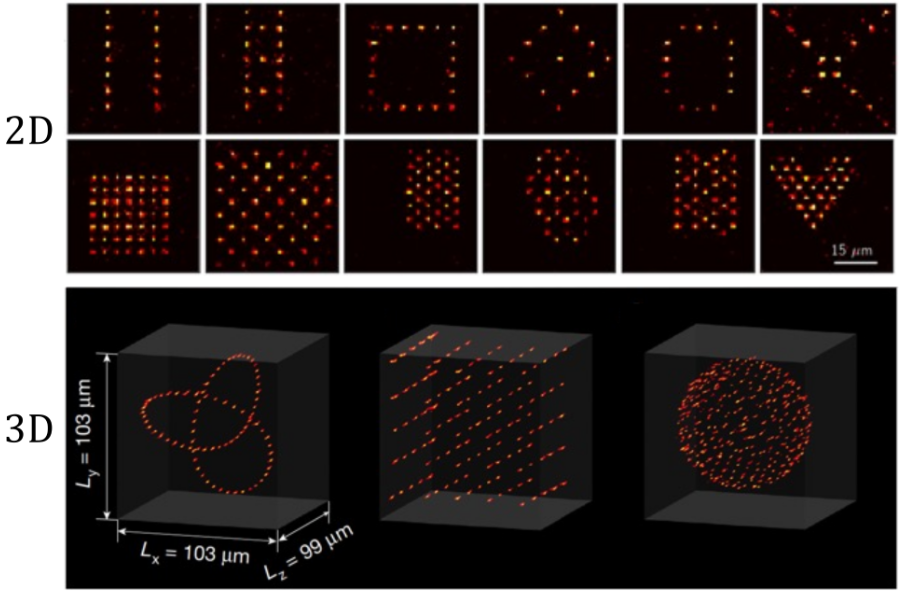
\includegraphics[width=0.8\textwidth]{img/2D-3D_neutral_atom_reg.png}
    \caption{2D and 3D neutral atom arrays. Image extracted from \cite{Henriet2020quantumcomputing}.}
    \label{fig:neutral_arrays}
\end{figure}

Unlike superconducting systems, where qubits are statically fabricated on a physical chip, neutral atoms can be dynamically arranged and manipulated using optical tweezers. This inherent flexibility allows for the creation of custom geometries and the implementation of specific interaction topologies between qubits, which is highly advantageous for solving optimization problems that demand tailored connectivity.

However, because the register is not permanently fixed, it must be reconstructed for each computation cycle. The overall execution process consists of three main phases:
\begin{itemize}
    \item Register preparation
    \item Quantum processing
    \item Register readout
\end{itemize}

The primary focus of this thesis, however, precedes the physical execution phase. It centers on the algorithmic challenge of efficiently embedding a QUBO problem onto this spatially constrained register to find optimal or near-optimal solutions. While the remainder of this work focuses mainly on the algorithmic approach, leveraging libraries and remote simulation infrastructures rather than delving into low-level hardware control, understanding the physical constraints of the QPU is essential. Therefore, following the explanations provided by \cite{Henriet2020quantumcomputing}, we briefly outline the physical mechanisms behind register loading and readout.

\paragraph{Register loading}
Configuring the atomic register requires a complex optical setup, relying on arrays of optical tweezers alongside the components illustrated in Figure \ref{fig:qpu_components}.

\begin{figure}[htbp]
    \centering
    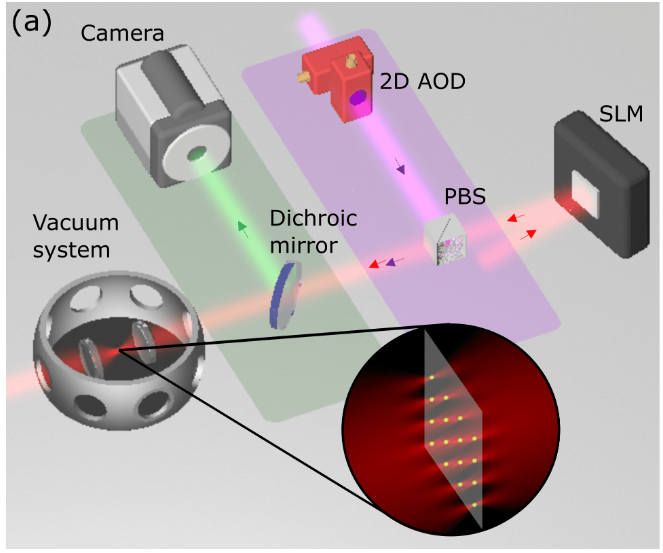
\includegraphics[width=0.8\textwidth]{img/principal_compo_QPU.png}
    \caption{Main hardware components of a neutral atom QPU. The trapping laser light (red) is shaped by a Spatial Light Modulator (SLM). Moving tweezers (purple), used to rearrange atoms, are controlled by a 2D Acousto-Optic Deflector (AOD) and superimposed using a Polarizing Beam-Splitter (PBS). The green fluorescence emitted by the atoms is separated by a dichroic mirror and captured by a camera during the readout phase. Image adapted from \cite{Henriet2020quantumcomputing}.}
    \label{fig:qpu_components}
\end{figure}

In essence, the process begins inside a vacuum chamber, where a laser system cools and confines a cloud of atoms. Subsequently, high-precision lenses focus light beams into extremely tight spots, creating optical tweezers. Each optical trap is designed to isolate and hold a single atom. By leveraging holographic techniques through a Spatial Light Modulator (SLM), it is possible to project these tweezers into predefined positions, generating the desired geometric array. This mechanism is the cornerstone of the technology's scalability: theoretically, scaling the system primarily requires increasing laser power and improving optical resolution to project more traps.

However, loading atoms from the cooled cloud into the traps is a stochastic process. Due to light-assisted collisions, each optical tweezer has roughly a 50\% probability of capturing exactly one atom, leaving the remaining traps empty. To construct a defect-free computational register, the system must perform an active rearrangement. This is achieved using dynamic tweezers governed by Acousto-Optic Deflectors (AODs), which sort and move atoms from filled traps into empty ones. This sorting process is repeated until the target array is completely filled, resulting in a perfect register ready for the quantum processing phase \cite{Henriet2020quantumcomputing}.

\paragraph{Quantum processing and register readout}

Once the atomic array is perfectly assembled, the quantum processing phase can begin. It is worth noting a significant timescale disparity in this hardware: while the actual quantum computation (performed via precisely timed laser pulses) is extremely fast, typically lasting less than 100 \textmu s, the entire computational cycle is dominated by the physical loading and readout phases, requiring approximately 200 ms in total \cite{Henriet2020quantumcomputing}.

After the algorithm is executed, the final state of the register must be measured to extract the classical solution. This readout phase is performed through fluorescence imaging. The physical system is tuned so that atoms remaining in the ground state (representing the logical qubit state $|0\rangle$) emit photons and appear as bright spots on the image. Conversely, atoms excited to the Rydberg state (representing the logical qubit state $|1\rangle$) do not fluoresce and remain dark. 

These optical signals are captured by highly sensitive Electron-Multiplying CCD (EMCCD) cameras. This detection method is extremely reliable, reaching readout efficiencies above 98.6\%, a performance highly competitive with the readout fidelities typical of superconducting circuits \cite{Henriet2020quantumcomputing}. Finally, due to the inherently probabilistic nature of quantum mechanics, a single execution yields only one possible classical bit-string. Therefore, the complete sequence of preparation, processing, and readout must be repeated hundreds or thousands of times (taking multiple \textit{shots}) to reconstruct the statistical probability distribution of the outcomes and successfully identify the optimal solution.

\paragraph{Quantum analog mode execution}

Neutral atom platforms can operate in both digital and analog modes. This work concentrates exclusively on the latter; please refer to \cite{Henriet2020quantumcomputing} for more information on the former. The dynamics of the analog mode are well-described by the Ising model, governed by the following Hamiltonian:

\begin{equation}
    \hat{\mathcal{H}}(t)=\hbar\sum_{i=1}^{N}\left(\frac{\Omega(t)}{2}\hat{\sigma}_{i}^{x}-\delta(t)\hat{n}_{i}\right)+\sum_{i<j}\frac{C_{6}}{|r_{i}-r_{j}|^{6}}\hat{n}_{i}\hat{n}_{j}
\end{equation}

This equation can be conceptually divided into two parts. The first summation dictates the evolution of single atoms driven by the external laser field, while the second summation governs the interactions between pairs of atoms. Specifically, the parameters and operators are defined as follows:
\begin{itemize}
    \item $N$ is the total number of atoms (qubits) in the register;
    \item $\Omega(t)$ is the time-dependent Rabi frequency, representing the amplitude of the laser exciting the atoms;
    \item $\delta(t)$ is the detuning parameter of the laser frequency;
    \item $\hat{\sigma}_{i}^{x}$ is the Pauli-X operator acting on atom $i$, which drives the transition between the ground state $|0\rangle$ and the Rydberg state $|1\rangle$;
    \item $\hat{n}_{i}$ is the occupation number operator (defined as $|1\rangle_i\langle 1|_i$) which evaluates to 1 if atom $i$ is in the Rydberg state, and 0 otherwise;
    \item $r_i$ is the spatial position of atom $i$;
    \item $C_6$ is the Van der Waals interaction coefficient, which is a constant dependent on the specific atomic species and platform used \cite{nowak2026satellitemissionplanningrydberg}.
\end{itemize}

Crucially, the third term in this Hamiltonian represents the interaction between individual spins. It accounts for the energy penalty incurred when two spatially close qubits occupy the Rydberg state simultaneously. When excited, qubits transition to the Rydberg state; however, if they are physically in close proximity, they experience the \textit{Rydberg blockade effect}. In this regime, maintaining the Rydberg state by the first qubit heavily suppresses the excitation of the second. Qubits in Rydberg states interact with each other proportionally to the third term above, following the Van der Waals potential for dipole-dipole interactions:

\begin{equation}
V_{ij} = \frac{C_6}{r_{ij}^6}
\end{equation}

where:
\begin{itemize}
    \item $V_{ij}$ is the interaction energy between atoms $i$ and $j$;
    \item $C_6$ is the Van der Waals coefficient, which depends on the atom type and scales massively with the excitation level;
    \item $r_{ij}$ is the spatial distance between the two atoms \cite{Henriet2020quantumcomputing}.
\end{itemize}
\chapter{The Embedding Problem: Theoretical Framework} \label{chap:embedding_problem}

This chapter introduces the theoretical framework behind the embedding problem for Neutral Atom Quantum Architectures. 
The aim of this part is to explain the complexity of finding efficient embeddings, starting with an introduction of basic concepts 
of computational complexity and graph theory, and then proceed to define Unit Disk Graphs (UDG) and the Maximum Independent Set (MIS) problem. Finally, these concepts will be connected to the current State of the Art (SOTA) and the Quadratic Unconstrained Binary Optimization (QUBO) formulation.


\section{Combinatorial Optimization and Computational and Geometrical Complexity}
\label{sec:combinatorial_opti_def}


Combinatorial optimization is a prominent branch of applied mathematics and computer science that focuses on finding an optimal object from a finite, discrete set of possible solutions. Specifically, the objective is to identify a solution that minimizes (or maximizes) a well-defined cost function, often subject to a set of strict mathematical constraints \cite{korte2012combinatorial}. 

These problems commonly involve discrete mathematical structures such as graphs, permutations, or boolean variables and are ubiquitous in fields ranging from logistics and network routing to machine learning and quantum physics \cite{papadimitriou1998combinatorial}. Although the solution space for these problems can be strictly finite, the number of possible configurations still can be overwhelmingly large. 

Moreover, combinatorial optimization frequently encounters $NP$-Hard problems, where finding the exact global optimum becomes computationally intractable. Consequently, the field heavily leverages heuristics and metaheuristics to find high-quality approximate solutions within a reasonable timeframe. Within this computationally demanding landscape, Quantum Computing emerges as a disruptive paradigm; by exploiting quantum mechanical phenomena, it promises to solve significantly larger $NP$-Hard instances and achieve higher-quality approximate solutions more efficiently than classical approaches \cite{memon2024quantum}.

Provided this general computational complexity, a secondary, equally formidable challenge arises when utilizing neutral atom platforms: the geometrical complexity. As introduced in Chapter \ref{chap:introduction}, executing an embedding algorithm requires mapping (or \textit{embedding}, precisely) the logical variables of the optimization problem onto the physical atoms arranged in a 2D or 3D register \cite{Henriet2020quantumcomputing}. 
In our specific case, focusing on a 2D plane, the hardware imposes strict geometric constraints and specific interaction boundaries governed by the Ising model and the Rydberg blockade. Finding an efficient spatial mapping that preserves the problem's theoretical connectivity while respecting these strict physical limitations is, remarkably, an $NP$-Hard problem in itself \cite{Vercellino_2022}.

\section{Unit Disk Graphs (UDG) and the Maximum Independent Set (MIS)}
\label{sec:UDG_and_MIS}

A graph can be formally denoted as:

\begin{equation}
    G = (V, E)
\end{equation}

where $V$ is the set of vertices (or nodes) and $E$ is the set of edges connecting them. Graphs are very common mathematical structures used to model relations between objects, and their properties are supported by a vast, historically established and robust theoretical foundation \cite{berge2001theory}. 

Thus, while an exhaustive review of graph theory is beyond the scope of this work, these structures will be briefly presented because of fundamental interest. Indeed, a significant portion of current literature focuses on graph-based combinatorial problems, primarily because graphs serve as the standard mathematical interface to encode and map optimization tasks onto quantum architectures. 
Prominent examples of such $NP$-Hard problems include the Maximum Cut (Max-Cut), the Traveling Salesperson Problem (TSP), and the Maximum Independent Set (MIS), which have extensively served as standard benchmarks for evaluating the performance of quantum algorithms \cite{lucas2014ising}.

To specialize our focus from general graphs, we introduce the concept of Unit Disk Graphs (UDG). As formalized by Clark et al. \cite{CLARK1990165}, UDGs can be defined through three mathematically equivalent geometric models:

\begin{itemize}
    \item \textbf{Distance Model:} Given a set of $n$ points in the Euclidean plane, a $n$-vertex graph is formed where each vertex corresponds to a point ($|V| = n$). An edge exists between two vertices if and only if the Euclidean distance $d(u, v)$ between the two corresponding points $u$ and $v$ is at most a specified threshold radius $r$. Mathematically, the edge set is defined as:
    \begin{equation}
        E = \{ \{u, v\} \mid u, v \in V, \; d(u, v) \leq r \}
    \end{equation}
    \item \textbf{Intersection Model:} Consider a set of $n$ equal-sized circles in the plane. The UDG is the intersection graph of these circles: each vertex corresponds to a circle, and an edge appears between two vertices if their corresponding circles overlap (tangent circles are also assumed to intersect).
    \item \textbf{Containment Model:} Alternatively, considering again $n$ equal-sized circles, an edge exists between two vertices if the circle corresponding to one vertex geometrically contains the center of the other.
\end{itemize}

\begin{figure}[htbp]
\centering
\begin{tikzpicture}[scale=1.5]
    % --- Pannello Sinistro: Distance Model ---
    \node at (1, 2.5) {\textbf{(a) Distance Model}};

    % definizione dei nodi (punti)
    \coordinate (A) at (0, 0);
    \coordinate (B) at (1.5, 0.5);
    \coordinate (C) at (0.5, 1.5);
    \coordinate (D) at (2.5, 1.2);

    % Disegno degli archi validi (distanza <= r)
    \draw[thick] (A) -- (B) -- (C) -- (A);
    \draw[thick] (B) -- (D);

    % Disegno di un arco non valido per mostrare che la distanza > r
    \draw[dashed, gray] (C) -- (D) node[midway, above right] {$> r$};

    % Etichetta della distanza <= r
    \draw[<->, red, thick] (A) -- (B) node[midway, below right] {$d \leq r$};

    % Disegno dei pallini dei nodi
    \filldraw (A) circle (2pt) node[below left] {$u$};
    \filldraw (B) circle (2pt) node[below] {$v$};
    \filldraw (C) circle (2pt) node[above] {$w$};
    \filldraw (D) circle (2pt) node[right] {$z$};

    % --- Pannello Destro: Intersection Model ---
    \begin{scope}[xshift=5cm] % Sposto tutto a destra di 5cm
    \node at (1, 2.5) {\textbf{(b) Intersection Model}};

    \coordinate (A2) at (0, 0);
    \coordinate (B2) at (1.5, 0.5);
    \coordinate (C2) at (0.5, 1.5);
    \coordinate (D2) at (2.5, 1.2);

    % Raggio dei cerchi (r/2)
    \def\rad{0.9}

    % Disegno i cerchi (le "aree di influenza")
    \draw[fill=blue!10, draw=blue, dashed] (A2) circle (\rad);
    \draw[fill=blue!10, draw=blue, dashed] (B2) circle (\rad);
    \draw[fill=blue!10, draw=blue, dashed] (C2) circle (\rad);
    \draw[fill=blue!10, draw=blue, dashed] (D2) circle (\rad);

    % Disegno gli archi dove i cerchi si sovrappongono
    \draw[thick] (A2) -- (B2) -- (C2) -- (A2);
    \draw[thick] (B2) -- (D2);

    \filldraw (A2) circle (2pt);
    \filldraw (B2) circle (2pt);
    \filldraw (C2) circle (2pt);
    \filldraw (D2) circle (2pt);
    \end{scope}
\end{tikzpicture}
\caption{The equivalent geometric representations of a Unit Disk Graph (UDG) adapted from \cite{CLARK1990165}. \textbf{(a)} The Distance Model connects nodes $u$ and $v$ if their Euclidean distance is $d \leq r$. \textbf{(b)} The Intersection Model places a disk of radius $r/2$ centered on each node; edges are formed exclusively where disks overlap.}
\label{fig:udg_models}
\end{figure}

Given any of these three definitions, the other two can be derived in linear time, demonstrating that they describe the exact same class of graphs. Historically, UDGs have proven to be an excellent mathematical framework for modeling broadcast and cellular networks, effectively resolving real-world problems such as frequency assignment and emergency signal routing \cite{CLARK1990165}. 

In the context of this thesis, the distance model is ''the elected'' model: replacing the generic threshold distance $r$ with the Rydberg radius ($R_b$) perfectly captures the physical interaction connectivity of neutral atoms in a quantum register.

As previously mentioned, the Maximum Independent Set (MIS) is a classic $NP$-Hard combinatorial optimization problem. While canonically formulated on general graphs, it holds massive relevance for our architecture because the problem famously remains $NP$-Hard even when restricted to Unit Disk Graphs \cite{CLARK1990165}.

Formally, given a graph $G = (V, E)$, an \textit{Independent Set} (IS) is defined as a subset of vertices $I \subseteq V$ such that no two vertices within $I$ are adjacent. Mathematically, this constraint translates to:
\begin{equation}
    \forall u, v \in I, \; u \neq v \implies \{u, v\} \notin E
\end{equation}
The MIS problem entails finding an independent set that contains the largest possible number of vertices; in other words, the objective is to maximize the cardinality $|I|$.

Given the aforementioned definitions, a straightforward and perfect isomorphism emerges between the abstract MIS problem on a UDG and the physical dynamics of neutral atom arrays. Specifically, the geometric threshold radius $r$ of the UDG corresponds directly to the Rydberg blockade radius ($R_b$). 

Consequently, the core mathematical constraint of the MIS problem, which strictly forbids selecting two adjacent vertices, is natively and physically enforced by the Rydberg blockade phenomenon, which prevents any two atoms within a distance $R_b$ from being simultaneously excited to the Rydberg state. 
Because of this perfect theoretical alignment, applying a global laser pulse designed to maximize the number of excited atoms in the 2D register forces the quantum many-body system to naturally evolve toward a ground state that inherently encodes the exact solution to the Maximum Independent Set of the corresponding geometric graph \cite{Henriet2020quantumcomputing}.
\begin{figure}[htbp]
\centering
\begin{tikzpicture}[scale=1.2]
    
    % Definizione del Raggio di Rydberg (Rb) e spaziatura griglia
    \def\Rb{1.6}
    
    % Nodi della soluzione MIS (Atomi eccitati)
    \coordinate (E1) at (0,0);
    \coordinate (E2) at (3,0);
    \coordinate (E3) at (6,0);
    \coordinate (E4) at (1.5, 1.5);
    \coordinate (E5) at (4.5, 1.5);
    \coordinate (E6) at (0, 3);
    \coordinate (E7) at (3, 3);
    \coordinate (E8) at (6, 3);

    % Disegno prima i cerchi del blocco di Rydberg (sfumati in sottofondo)
    \foreach \p in {E1, E2, E3, E4, E5, E6, E7, E8} {
        \fill[red!15] (\p) circle (\Rb);
        \draw[red!50, dashed] (\p) circle (\Rb);
    }

    % Disegno gli archi del grafo UDG in modo corretto e nativo
    \draw[gray!30, thick, step=1.5] (0,0) grid (6,3);

    % Disegno tutti gli atomi neutri (Stato base, in nero)
    \foreach \x in {0, 1.5, 3, 4.5, 6} {
        \foreach \y in {0, 1.5, 3} {
            \filldraw[black] (\x,\y) circle (2.5pt);
        }
    }

    % Sovrascrivo gli atomi eccitati (Stato di Rydberg, in rosso e più grandi)
    \foreach \p in {E1, E2, E3, E4, E5, E6, E7, E8} {
        \filldraw[red] (\p) circle (3.5pt);
    }

    % Raggio 
    \draw[<->, thick] (E4) -- ++(\Rb,0) node[midway, above, font=\footnotesize] {$R_b$};

\end{tikzpicture}
\caption{Physical realization of the Maximum Independent Set (MIS) via the Rydberg blockade. Red dots represent atoms excited to the Rydberg state (\textbf{MIS selected nodes}), while black dots are atoms remained in the ground state (\textbf{unselected nodes}). 
The shaded red regions represent the Rydberg blockade volume (radius $R_b$). The physical mechanism preventing two Rydberg excitations from overlapping perfectly enforces the mathematical constraint of the MIS problem.}
\label{fig:rydberg_mis}
\end{figure}

\section{Literature and State of the Art}
\label{sec:SOTA}

Defining a definitive State of the Art (SOTA) for the embedding problem on neutral atom architectures is challenging, as the field remains at the absolute frontier of quantum computing research. Presently, there is no universally established protocol or singular ``gold standard'' architecture. Instead, the literature presents a diverse landscape of experimental approaches and heuristic strategies aimed at overcoming the strict geometric constraints of these platforms.

To illustrate this dynamic ecosystem, recent literature explores a wide array of embedding techniques. For instance, Vercellino et al. \cite{Vercellino_2022} investigate the use of Neural Networks to dynamically map problem graphs onto physical registers. Other approaches rely on force-directed heuristics; notably, Tarquini et al. \cite{tarquini2026dronedeliverypackingproblem} successfully (within a reasonable dimension less than circa 50 nodes) experimented with the Fruchterman-Reingold (FR) algorithm, enhanced by sophisticated pre- and post-processing techniques, 
to embed Quadratic Unconstrained Binary Optimization (QUBO) problems.

Alongside embedding algorithms, significant research is devoted to translating highly complex real-world use cases into physical layouts. Examples include the formulation of emergency hub placement routing \cite{tarquini2026emergencyhubplacementneutralatom} and satellite mission planning \cite{nowak2026satellitemissionplanningrydberg}, demonstrating the vast applicability of QUBO formulations on neutral atoms.


Most importantly for this thesis, several recent studies have started exploring advanced mapping and partitioning techniques as a workaround for hardware scale limitations. Works by Nembrini et al. \cite{nembrini2024application, Nembrini_2026} propose innovative Reinforcement Learning methodologies to tackle the severe embedding bottlenecks inherent to quantum annealing topologies. On the other hand, focusing strictly on neutral atom architectures, Das et al. \cite{das2025grid} explicitly propose problem partitioning, dividing the original combinatorial problem into sub-instances resolved using localized atomic arrays. While their specific methodologies differ from our scope, these partitioning strategies served as the foundational inspiration for the hybrid \textit{divide et impera} (divide and conquer) architecture proposed in the subsequent chapters of this work.

This diversity of approaches underscores the immaturity and the highly exploratory nature of the field. While the lack of rigid standards offers significant opportunities for novel theoretical contributions, it also introduces substantial experimental risks and engineering bottlenecks. 

Drawing from this extensive body of literature, we chose to restrict our focus specifically to the QUBO mathematical framework, which will be formally defined in the next section. More importantly, mainly driven by the operational realities and constraints of the currently available experimental platforms, our investigation will target QUBO instances that naturally exhibit a UDG-like connectivity. This specific focus bypasses the need for massive auxiliary embeddings, setting the optimal stage for our distributed algorithmic approach.


\section{Quadratic Unconstrained Binary Optimization (QUBO)}
\label{sec:QUBO}

Quadratic Unconstrained Binary Optimization (QUBO) provides a unifying mathematical framework for modeling a vast array of combinatorial optimization problems. As the name suggests, this formulation strictly involves binary decision variables and a quadratic objective function, notably without imposing any external algebraic constraints. 

This formulation has gained immense popularity across various scientific and industrial fields due to its remarkable versatility. As demonstrated in comprehensive tutorials \cite{glover2018tutorial}, a multitude of classically constrained problems (such as the TSP, Max-Cut, or Graph Coloring) can be seamlessly recast into the unconstrained QUBO format through the use of penalty terms. Consequently, a massive segment of modern literature focuses on QUBO as the standard input format for quantum platforms. While historically popularized by quantum annealing systems built on superconducting qubits (such as D-Wave \cite{QUBO-D-Wave}), QUBO is increasingly becoming the target formulation for neutral atom architectures as well \cite{nowak2026satellitemissionplanningrydberg, Vercellino_2022, das2025grid}.

From a formal mathematical perspective, solving a QUBO problem entails finding the specific assignment of a binary vector $x$ that minimizes (or maximizes, note that a minimization problem is equivalent to a maximization one by simply applying a minus sign ($-$) to the objective function) a quadratic cost function:

\begin{equation}
    \min_{x \in \{0,1\}^n} f(x) = x^T Q x = \sum_{i=1}^{n} \sum_{j=1}^{n} Q_{i,j} x_i x_j
\end{equation}

where:
\begin{itemize}
    \item $x = (x_1, x_2, \dots, x_n)$ is a vector of $n$ binary decision variables;
    \item $Q$ is an $n \times n$ square matrix of real constants detailing the problem's costs and interactions.
\end{itemize}

A key mathematical property of binary variables is that $x_i^2 = x_i$ for any $x_i \in \{0,1\}$. This elegantly allows any linear term of the objective function to be mapped directly onto the main diagonal of the $Q$ matrix ($Q_{i,i}$), while the off-diagonal elements ($Q_{i,j}$ for $i \neq j$) encode the quadratic interactions, or "penalties," between pairs of variables.

Our decision to adopt the QUBO framework for investigating hybrid embedding methodologies is twofold. First, it ensures broad applicability across the wide variety of problems identifiable in the literature \cite{glover2018tutorial}. Second, and most crucially, the binary nature of the variables establishes a native, one-to-one mapping with the physical states of a quantum register: each variable $x_i \in \{0,1\}$ directly dictates whether a specific atom $i$ is left in the ground state ($|0\rangle$) or excited to the Rydberg state ($|1\rangle$). This elegant bridge between mathematical abstraction and hardware execution perfectly sets the stage for the algorithmic development detailed in the next chapter.

\paragraph{Investigated QUBO Instances}
Due to specific hardware and simulator constraints, the experimental phase of this work focuses exclusively on UDG-like QUBO matrices. Specifically, we evaluate randomly generated QUBO instances whose underlying interaction connectivity strictly mirrors the geometric topology of a Unit Disk Graph.

Furthermore, to ensure physical compatibility with current neutral atom platforms, these matrices are constrained to exhibit uniform parameter distributions. All elements on the principal diagonal are assigned identical values; mathematically, this uniform linear cost reflects the hardware limitation of employing a global driving laser, which applies the same detuning and Rabi frequency uniformly across the entire atomic register. Similarly, all non-zero off-diagonal elements share a constant penalty value, effectively representing the uniform, binary nature of the Rydberg blockade interaction across all valid UDG edges.



\chapter{The Base Pipeline and its Limits} 
\label{chap:base_pipeline}

This chapter presents the baseline architecture of our embedding pipeline and the related experimental results. The purpose is to detail how the embedding problem was methodologically approached, which embedding optimization methods were selected and tested, and what scalability limitations  and fitness scores emerged. Finally, will be discussed how these limitations are natively imposed by the interplay between the mathematical formulation and the specific hardware constraints of the target quantum platform.

\section{Base pipeline: conceptual scheme}
\label{section:conceptual_base_pipeline}

\begin{figure}[htbp]
    \centering
    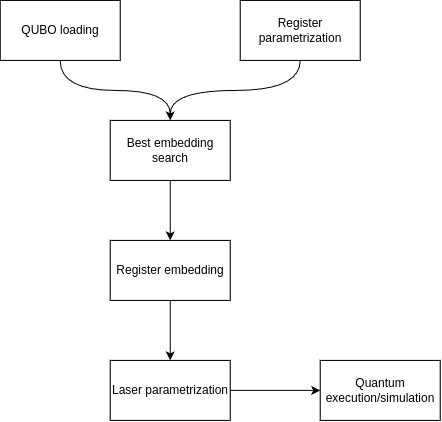
\includegraphics[width=0.5\textwidth]{img/base_pipeline.png} 
    \caption{Flowchart of the basic pipeline. The process highlights an hybrid classical-quantum approach.}
    \label{fig:base_pipeline}
\end{figure}

As illustrated in the conceptual scheme in Figure \ref{fig:base_pipeline}, the first operational phase of the pipeline requires loading the QUBO problem instance. Therefore, it is strictly necessary to detail the geometric and mathematical characteristics of the investigated instances, as well as the hardware restrictions that dictated their generation.

\subsection{Hardware Constraints and the Jülich HPC Emulator}
As discussed, neutral atom platforms present some physical limitations. The most impactful constraint for our formulation is the reliance on a \textit{global driving laser}, which uniformly illuminates the entire atomic register and so imposes the impossibility to excite differently different atoms or clusters of different atoms. Mathematically, this enables a feasible quantum execution only for QUBO matrices that exhibit uniform values on the principal diagonal (representing a constant linear cost/detuning) and uniform off-diagonal penalties (representing the binary Rydberg blockade).

In order to emulate as much as possible a real-world applicability of this thesis, the pipeline was explicitly designed to target \textbf{Jade}, a state-of-the-art Neutral Atom Quantum Processing Unit \cite{pasqal2026italy}. While we initially planned for physical execution on it, access to the actual Jade hardware was postponed to the upcoming December due to broader availability constraints. Consequently, the experimental phase for the moment has relied to a remote analog quantum emulator provided by the \textbf{Jülich Supercomputing Centre (JSC)} in Germany. 

To ensure that the research performed remains perfectly forward-compatible with the real machine once available, we injected a custom hardware profile into the simulator (referred to in the codebase \cite{orsucci_qubo_ga_quantum} as \texttt{FakeJade}). This profile strictly enforces Jade's actual physical parameters in order to be able to directly test this work on it in the near future.


The \texttt{FakeJade} physical profile injected into the emulator severely bounds the degrees of freedom available to the classical embedding algorithm. Extracting directly from platform API call, the hardware constraints are the following:

\begin{itemize}
    \item \textbf{Maximum Radius ($R_{max}$):} The entire atomic register must be confined within a specific continuous area dictated by the laser focusing limits. For our emulator, the coordinates confined within a circular plane with a maximum radius of $R_{max} = 50.0\,\mu\text{m}$.
    
    \item \textbf{Minimum atomic distance ($d_{min}$):} Due to the diffraction limits of the optical tweezers, two atoms cannot be placed arbitrarily close or overlapped (we are considering a 2D register). The hardware enforces a minimum inter-atomic distance of $d_{min} = 4.0\,\mu\text{m}$. Breaching this threshold causes a hard physical violation and the impossibility to submit the task to remote infrastructure.
    
    \item \textbf{Interaction Saturation ($V_{max}$):} Neutral atoms interact following the Van der Waals potential ($V = C_6 / r^6$), the combination of physical laws and the $d_{min}$ constraint, caps the maximum possible interaction strength between any two qubits. The highest tolerable penalty in the system is saturated at $V_{max} = C_6 / d_{min}^6$.
    
    \item \textbf{Global Channel Energetics and Scaling:} The QPU operates via a single \texttt{rydberg\_global} channel. This imposes ceilings on the maximum allowable Rabi frequency ($\Omega_{max}$) and the maximum absolute detuning ($|\delta|_{max}$). Because raw QUBO weights can mathematically exceed these physical capacities, the embedding pipeline must calculate a restrictive \textit{Scale Factor}. As implemented in the codebase \cite{orsucci_qubo_ga_quantum}, the entire QUBO matrix is dynamically (instance per instance) scaled down by a factor of $\min(\frac{V_{max}}{\max(Q_{off-diagonal})}, \frac{|\delta|_{max}}{\text{avg}(Q_{diagonal})})$ to ensure the problem fits within the hardware's physical energy envelope.
\end{itemize}

\subsection{QUBO Instance Generation}
These strict hardware parameters played a foundational role in how the test datasets were generated. To guarantee that the problem instances are physically embeddable on the targeted neutral atom architecture, a specialized Python generation script was developed. Rather than generating arbitrary random graphs, the script synthesizes ``verisimilar'' Unit Disk Graphs (UDG) by simulating the actual physical placement of atoms under the constraints aforementioned.
The generation logic is composed by the following procedural steps:
\begin{enumerate}
    \item \textbf{Dynamic Operational Area Calculation:} To achieve a specific target average degree (which dictates primarly the problem's difficulty), an effective operational radius is dynamically calculated. This radius scales proportionally with the square root of the number of nodes ($N$) and the Rydberg radius. Most important, it is mathematically bounded to never exceed the physical limits of the machine (the $50\,\mu\text{m}$ maximum hardware radius) while remaining large enough to accommodate all atoms.
    \item \textbf{Rejection Sampling Placement:} Node coordinates are generated uniformly within the operational area using polar coordinates. An hardware aware minimum-distance check is enforced during this process: any randomly generated position that falls within the minimum allowed optical trap distance ($d_{min} = 4.0\,\mu\text{m}$) of an already placed atom is immediately rejected. This ensures the resulting spatial configuration respects the optical tweezers' constraints.
    \item \textbf{QUBO Matrix Construction:} Once all $N$ coordinates are successfully placed within the delimited continuous space, the pairwise Euclidean distance matrix is computed. The QUBO matrix ($Q$) is then populated: all main diagonal elements are uniformly set to $-1.0$ (representing the global laser's tendency to drive the atoms toward the Rydberg state), and a constant penalty weight of $2.0$ is assigned to any off-diagonal edge where the inter-atomic distance is strictly less than the specified Rydberg blockade radius set ($R_b = 12.0\,\mu\text{m}$).
    \item \textbf{Data Serialization:} Finally, the non-zero upper triangular elements of the QUBO matrix are extracted and serialized into a (\texttt{.npz}) format. Although the original geometrically valid coordinates are stored for validation purposes, the embedding pipeline receives only the abstract mathematical weights (otherwise all of the next experimentations do not makes much sense), forcing the selected embedding algorithm to reconstruct a valid physical layout from scratch.
\end{enumerate}

\begin{figure}[htbp]
    \centering
    
     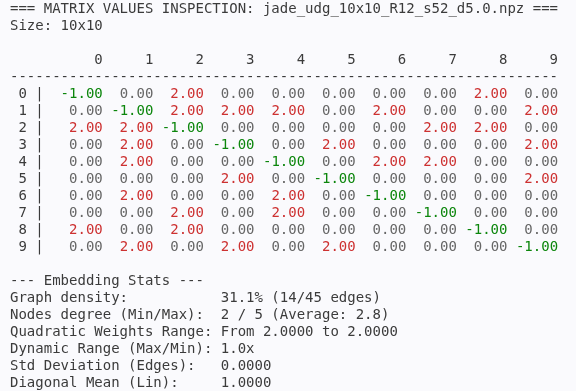
\includegraphics[width=0.6\textwidth]{img/QUBO_example.png} 
    \caption{Example of a small-scale UDG-like QUBO instance generated using the \textit{instance\_generator.py} as described above and inspected via \textit{inspect\_qubo.py} in \cite{orsucci_qubo_ga_quantum}.}
    \label{fig:qubo_generation_example}
\end{figure}

\subsection{Instance Loading and Matrix Parsing}
Once generated, the QUBO matrices and their metadata are compressed and stored in NumPy's binary format (\texttt{.npz}). As depicted in the first block of the pipeline flowchart, the execution begins with the \texttt{QUBO loading} module. 

A dedicated parser function extracts the indices and weights from the \texttt{.npz} file and reconstructs the symmetric $N \times N$ matrix ($Q$). Simultaneously, the system isolates the off-diagonal terms to calculate the maximum theoretical connectivity. 

\section{Embedding Optimization using Genetic Algorithms (GA)}
\label{sec:ga_optimization}

The search for an optimal physical embedding is a $NP$-Hard task characterized by a highly complex, non-convex optimization scenario that makes very ineffective using classical optimization methods such as the Nelder-Mead simplex method. As formalized in the previous section, among the challenges, we have that the computational engine must simultaneously satisfy strict geometric boundaries ($R_{max}$) and discrete proximity constraints ($d_{min}$) for example, all while minimizing in some way the topological error between the physical Van der Waals interactions and the mathematical QUBO penalties in order
to achieve a good enough fitness score and consequently (at least in principal) a good enough embedding.

Given the severity of these constraints and the complete lack of \textit{a priori} analytical information regarding the optimal spatial distribution of the atoms, we choose to initiate our experimental phase by testing a black-box, derivative-free optimization approach: Genetic Algorithms (GAs). This section has the main goal
to explain the main GAs' characteristics finalized to better contextualize the more attentioned experimental results.  


%ancora da ricontrollare
\paragraph{Genetic Algorithm Framework}
Genetic Algorithms represent a prominent branch of evolutionary computation, heavily inspired by the biological principles of natural selection and genetics. The possible different methodological classifications and terminologies are very different and influenced by the different biological and evolutionary elements inspiring the different algorithms, 
but in general they are particularly well-suited for optimization problems where the search space is discontinuous and when we don't have a priori information at all.

In our specific context of application, as a result of deep and complete study of \cite{bookGA}, considered the bible for Genetic Algorithms, we decided to design our GA with the following key aspects: 

\begin{itemize}
    \item an individual or chromosome in the GA population is a set of 2 continue 2D coordinates $(x,y)$ having a 2D register. A set for every $N$ atoms (binary variables).
    \item the population is iteratevely improved via crossover, parenting, selection...
    \item the population evalutation and improvement is done using a fitness function score as metric.
\end{itemize}

%continuare con esempio di configurazione GA
%spiegare nel dettaglio perchè è stata fatta questa scelta
%spiegare con esempio la fitness function, formalizzarla e spiegare perchè è stata scelta.
%\include{chapters/04_Distributed_Architecture}
%\include{chapters/05_Results}
%\include{chapters/06_Conclusions}

%--------------- Bibliografia ---------------
\addcontentsline{toc}{chapter}{Bibliography} % Corretto da 'Bibliografia' a 'Bibliography'
\bibliographystyle{ieeetr} % ieeetr è il formato standard per Ingegneria (numerato in ordine di citazione)
\bibliography{files/biblio} 

\end{document}